\subsection{查询条目(查)}

\paragraph{子查询} 子查询的设计会较大程度上的影响DBMS的性能,因为与其余常规查询操作不同,子查询一般无法被优化器综合性的优化进整体查询中。
\begin{lstlisting}
SELECT s.id, s.name
FROM project1.student s
WHERE s.college = (SELECT id FROM project1.college WHERE college.name = '格兰芬多')
  AND s.sex = 'M';
\end{lstlisting}
\vspace{-2em}
\par 在查询格兰芬多的所有男生信息时,使用子查询每次平均耗时0.308s,而查询书院编号及按编号查询数据的两个查询总耗时平均0.221s,这是因为类似于编程中的函数调用栈,当出现子查询时,查询器需要先保存上下文并跳转执行子查询,再将查询结果返回给“调用栈”的上一级查询任务。\\~\\
\centerline{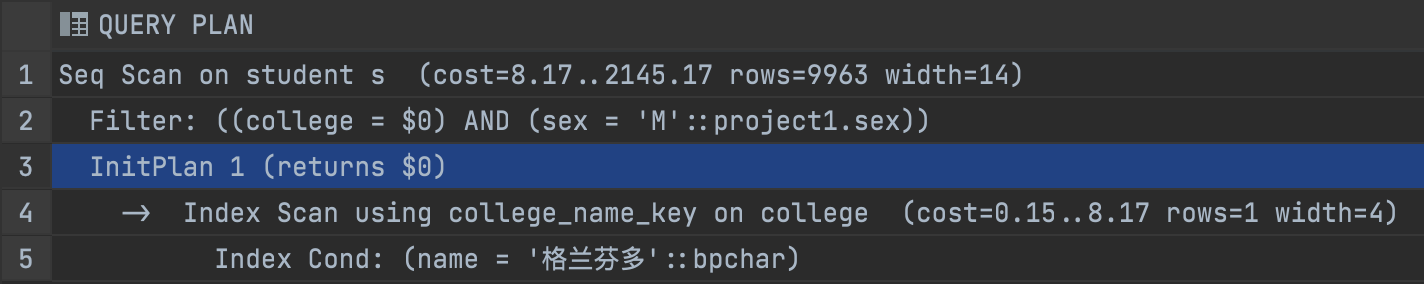
\includegraphics[width=0.9\textwidth]{dta/qp}}

\paragraph{索引} \par Index的设计能大大提升查询的性能。不使用index时,为了检查where子句中的条件,DBMS必须遍历整个表格中的所有行,并从众多列中选出其需要的部分,而为常用查询的条件部分设置index使得DBMS只需检查部分字段,大大减少了需要处理的信息量。
\begin{lstlisting}
SELECT sch_id
FROM project1.schedule
WHERE starting = 3
  AND ending = 4;
\end{lstlisting}
\vspace{-2em}
\par 在执行此查询时,该表上仅有数据库在设置主键列时自动添加的index,整表一共七个字段,而查询只涉及四个(且无完全包含查询所需字段的index),故需要提取每行的所有信息,耗时43ms。下面我们为查询涉及字段添加index,再次查询仅需15ms。此时DBMS在序列扫描数据时不需要提取全表信息,仅分析了sch\_time\_idx中包含的较少信息。更多关于索引的内容将于下文讨论。
\begin{lstlisting}
CREATE INDEX sch_time_idx ON project1.schedule (sch_id, starting, ending);
\end{lstlisting}
\vspace{-2em}
\paragraph{并行执行}
\par 并行化语句的执行过程会被规划器分发给多个后台进程去执行。 通过这种并行执行方式,PostgreSQL能充分发挥多核处理器的威力,从而让语句执行更快完成。通过并行化执行所能节省的时间根据数据库载体机的CPU核数的多寡而有所不同,在机器性能强大的情况下,并行化所能带来的性能提升可能非常可观。但是在查询任务数据量较少时,强制的并行化执行可能反而延长查询耗时——当每个进程所分配到的子任务规模较小时,创建worker的时间开销甚至大于执行查询的时间开销。
\par 通过下面的命令可以强行开启并行化执行模式,对比下例查询,使用1 worker时查询用时1.906s,并行化任务为其分配2 workers(如下图explain所示),耗时1.308s。
\begin{lstlisting}
SET force_parallel_mode = TRUE;
\end{lstlisting}
\vspace{-2em}
\begin{lstlisting}
SELECT course, COUNT(*)
FROM project1.learnt
GROUP BY course;
\end{lstlisting}
\vspace{-2em}
\centerline{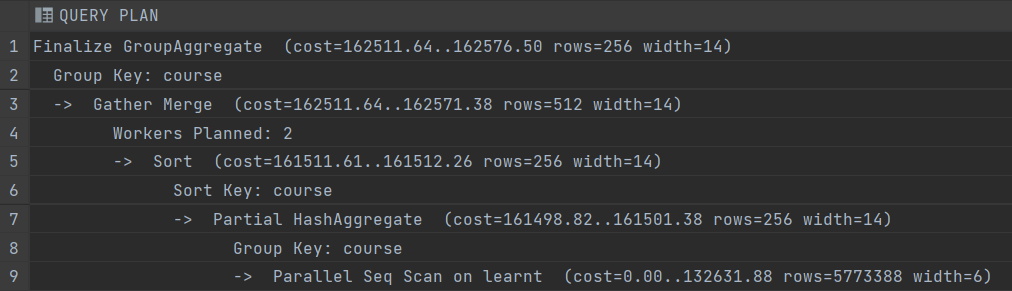
\includegraphics[width=0.8\textwidth]{dta/parall}}

\paragraph{where条件数} 若每层条件筛选后并不会大幅度减少剩余条目数量时,筛选条件越多,查询结果中剩余的项目分摊的执行时间越多,查询越慢。下例中标注的耗时指在原有条件的基础上增加此条件的耗时。
\begin{lstlisting}
SELECT sch_id
FROM project1.schedule
WHERE starting = 3 -- execution: 8ms
  AND ending = 4   -- execution: 9ms
  AND weekday = 3; -- execution: 11ms
\end{lstlisting}
\vspace{-2em}
